
\section{Game module}

The game is made in the Unity environment. It belongs to the tower defense type. The game board consists of tiles, which are three-dimensional models divided into two categories: ground and road. There is one ground tile and five road tiles (fig.~\ref{Fig:tiles}).

\begin{figure}
\begin{tikzpicture}
\node[anchor=center,inner sep=0, label=below:{Ground}] at (-4,3) {
\includegraphics[width=2cm]{images/tileGround.png}};
\node[anchor=center,inner sep=0, label=below:{Water}] at (-4,1) {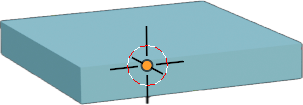
\includegraphics[width=2cm]{images/tileWater.png}};
\node[anchor=center,inner sep=0,label=below:{Straight}] (tikz) at (-1.5,1) {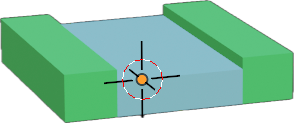
\includegraphics[width=2cm]{images/tileWaterStraight.png}};
\node[anchor=center,inner sep=0,label=below:{Curve}] (tikz) at (1,1) {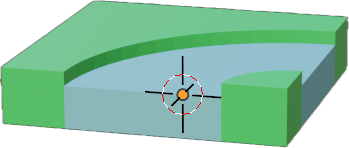
\includegraphics[width=2cm]{images/tileWaterCurve.png}};
\node[anchor=center,inner sep=0,label=below:{Intersection 1}] (tikz) at (3.5,1) {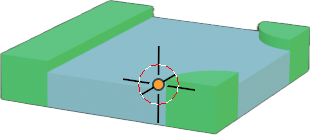
\includegraphics[width=2cm]{images/tileWaterIntersection1.png}};
\node[anchor=center,inner sep=0,label=below:{Intersection 2}] (tikz) at (6,1) {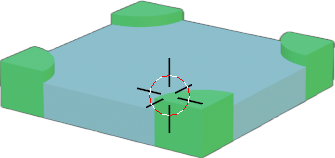
\includegraphics[width=2cm]{images/tileWaterIntersection2.png}};
\end{tikzpicture}

\caption{Tile models}
\label{Fig:tiles}
\end{figure}  

The figure~\ref{Fig:changeTiles} shows where in the Unity editor interface you should change the tile models (if necessary). The top selection shows where the earth tile model changes. The lower selection shows where the first road tile model was changed. The rest are in WaterStraight, WaterCurve, etc. The WaterBegin, WaterBeginEnd, etc. elements are combinations of the models in Figure~\ref{Fig:tiles} with arrows.

\begin{figure}
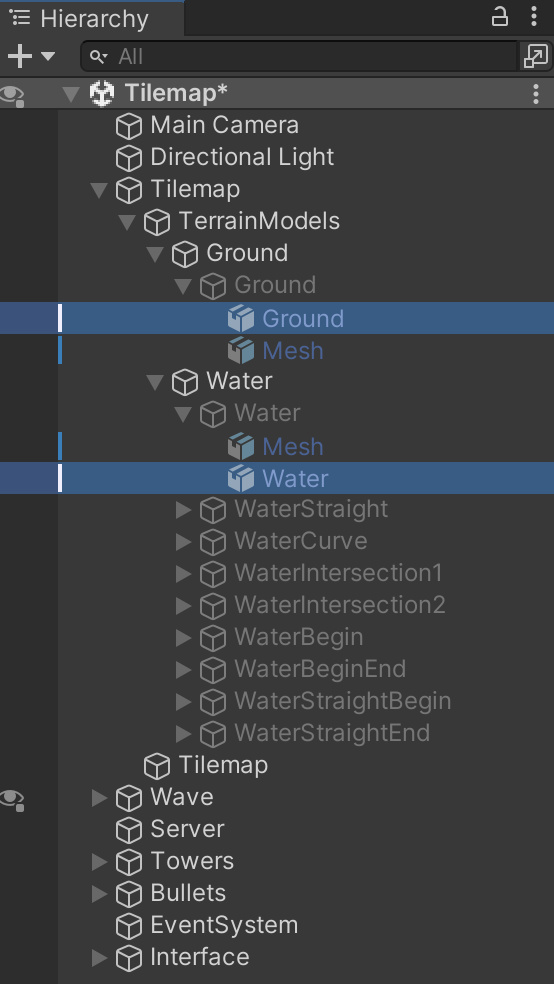
\includegraphics[width=5cm]{images/changeTiles.png}
\caption{Changing tile models}
\label{Fig:changeTiles}
\end{figure}  

Similarly, you can change the models of opponents and towers. The location of model changes is shown in Figures ~\ref{Fig:changeEnemy} and ~\ref{Fig:changeTower}.

\begin{figure}
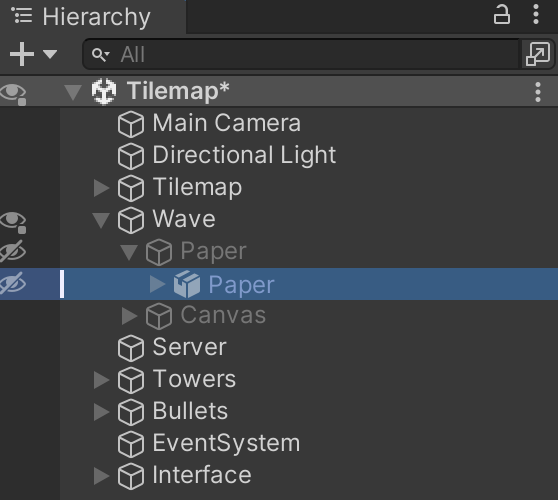
\includegraphics[width=5cm]{images/changeEnemy.png}
\caption{Changing the opponent's model}
\label{Fig:changeEnemy}
\end{figure}  


\begin{figure}
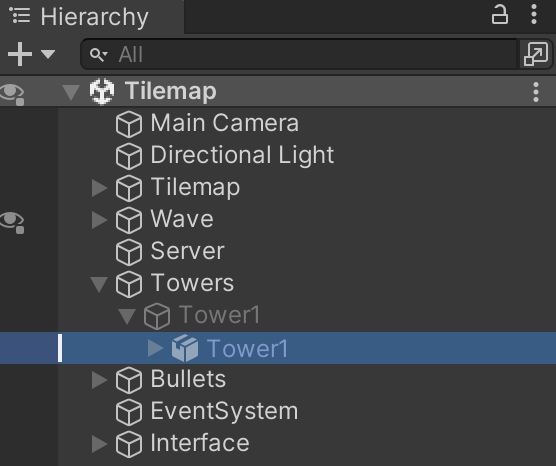
\includegraphics[width=5cm]{images/changeTower.png}
\caption{Changing the tower model}
\label{Fig:changeTower}
\end{figure}  

Figure~\ref{Fig:enemyParameters} shows the place where you can change enemy parameters in the Unity editor:
\begin{itemize}
\item Speed -- movement speed,
\item Start health -- start health,
\item Armor -- value subtracted from the damage dealt (causes invulnerability to bullets that have a lower amount of damage than Armour),
\item Coins -- number of coins needed to create an opponent,
\item Destroy Coins -- the number of coins that towers receive for killing an opponent,
\item Coins To End -- the number of coins that opponents receive if the opponent reaches the end point,
\item Count -- number of available opponents (-1 means unlimited number of opponents).
\end{itemize}

\begin{figure}
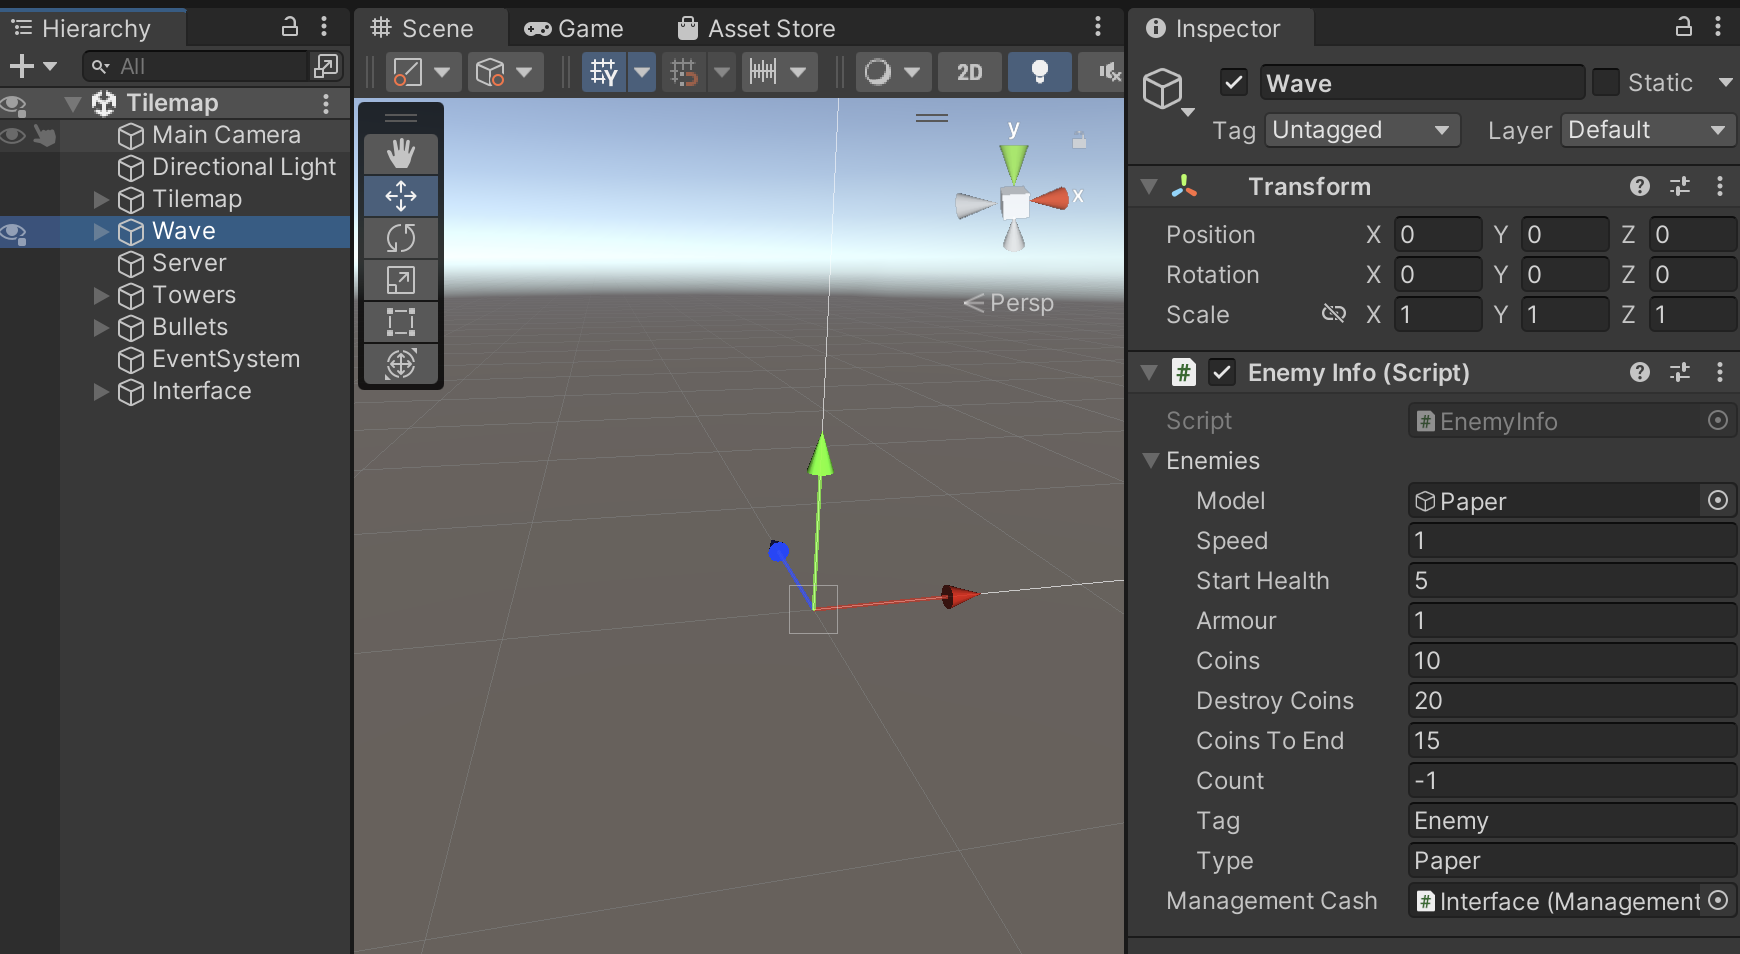
\includegraphics[width=15cm]{images/enemyParameters.png}
\caption{Changing opponents' parameters}
\label{Fig:enemyParameters}
\end{figure}  

Figure~\ref{Fig:towerParameters} shows the place where you can change tower parameters in the Unity editor:
\begin{itemize}
\item Speed -- rotation speed,
\item Rate From Fire -- rate of fire,
\item Bullet Strength -- number of damage dealt,
\item Force -- the force of firing the projectile that translates into its range,
\item Coins -- number of coins needed to create a tower,
\item Count -- number of available towers (-1 means unlimited number of towers).
\end{itemize}

\begin{figure}
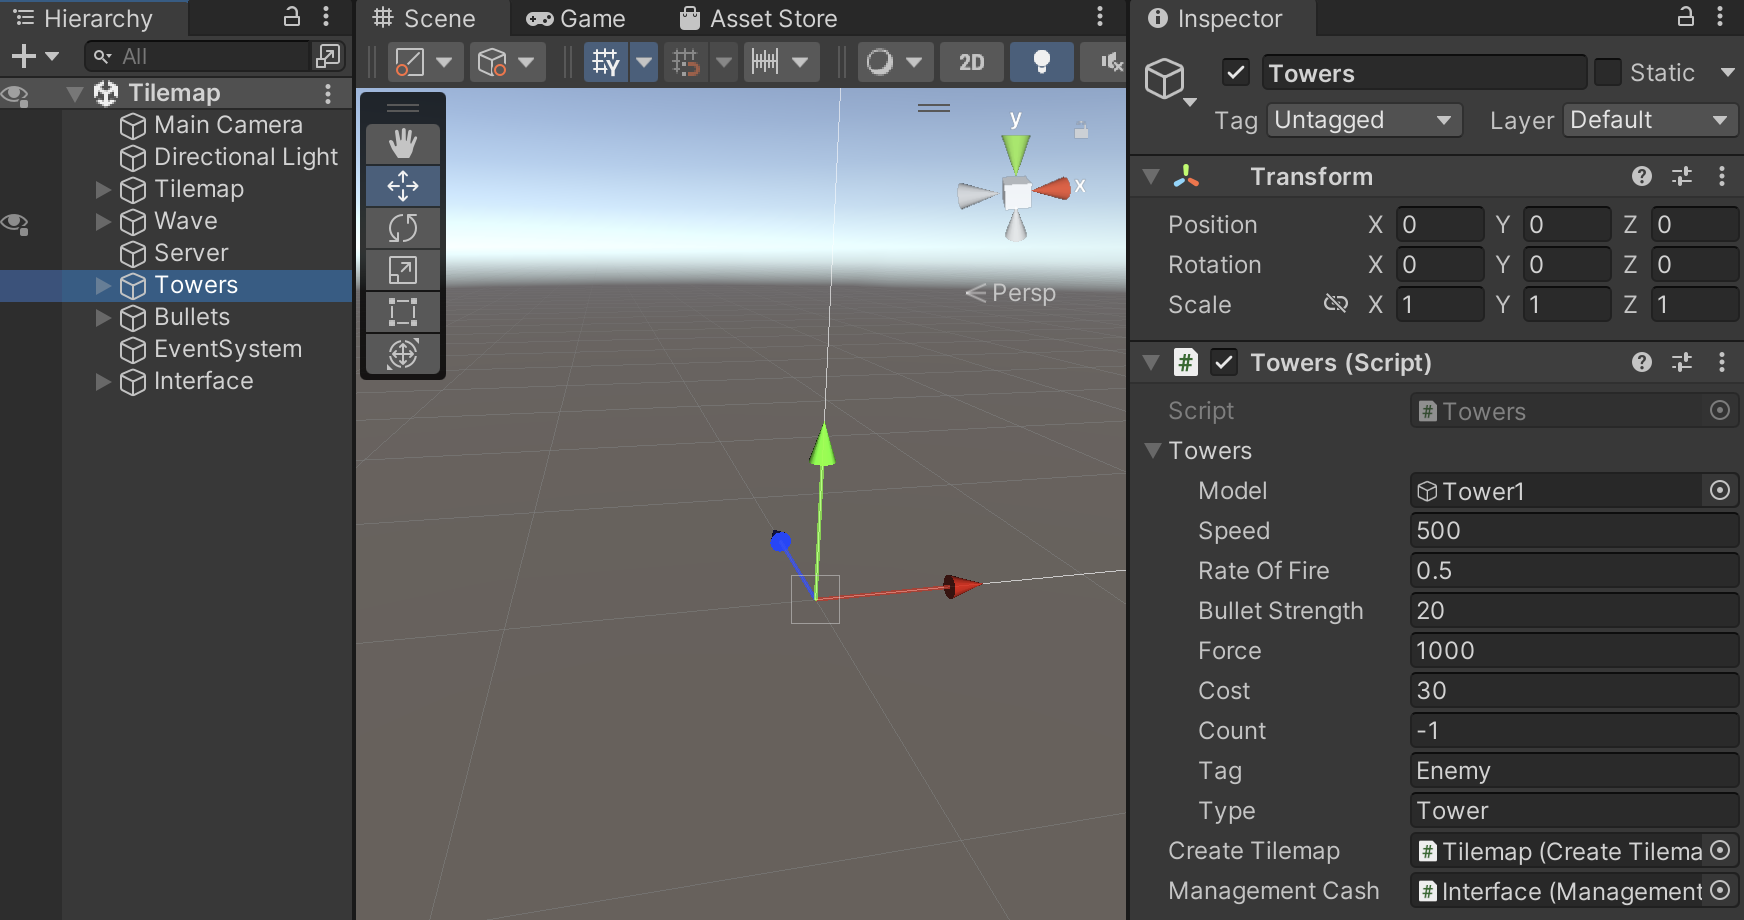
\includegraphics[width=15cm]{images/towerParameters.png}
\caption{Changing tower parameters}
\label{Fig:towerParameters}
\end{figure}  

Figure~\ref{Fig:startCoins} shows where you can change the starting number of coins in the Unity editor:
\begin{itemize}
\item Start Coins -- initial number of tower coins;
\item Start Enemy Coins -- the initial number of enemy coins.
\end{itemize}


\begin{figure}
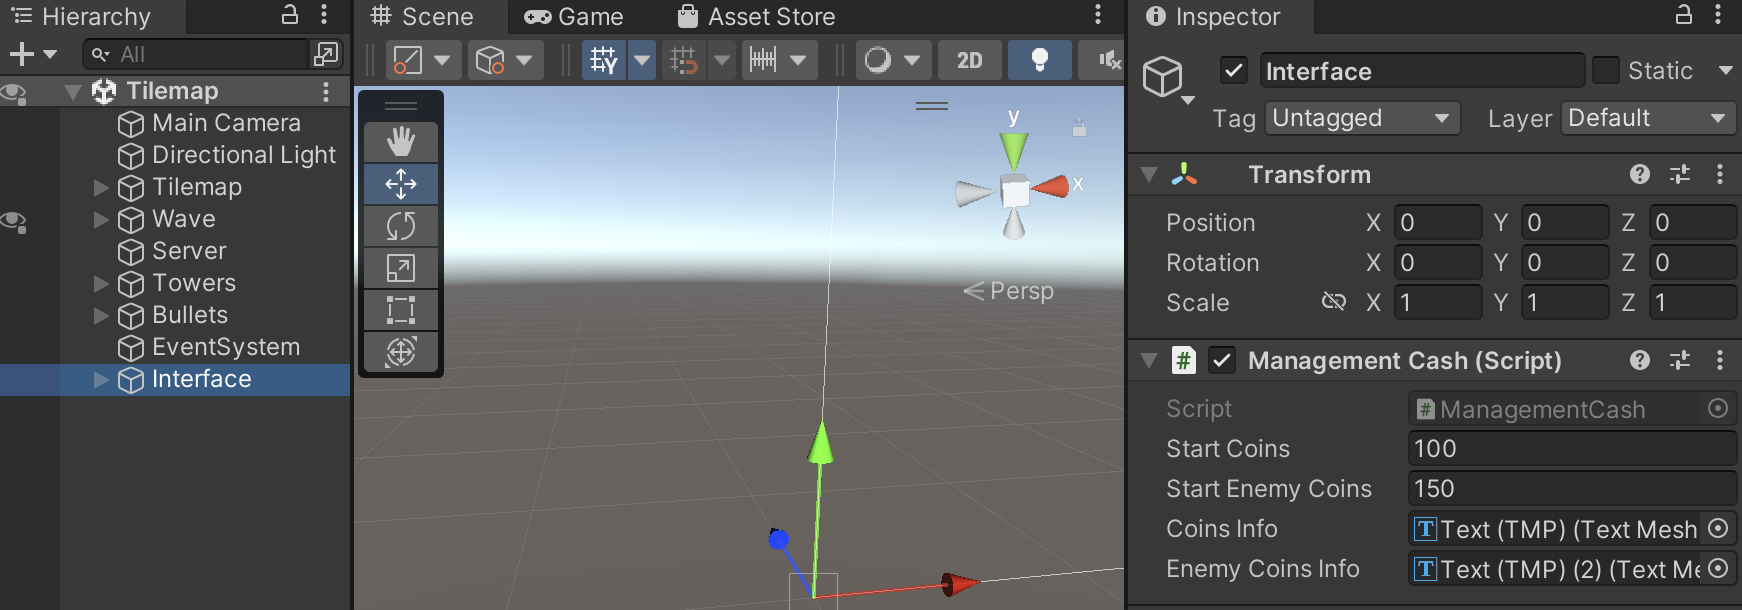
\includegraphics[width=15cm]{images/startCoins}
\caption{Starting coins}
\label{Fig:startCoins}
\end{figure} 

Figure~\ref{Fig:serverParameters} shows the place where you can change server parameters in the Unity editor:
\begin{itemize}
\item IP Address -- server IP address (127.0.0.1 means that the server will only be available to software installed on the same computer as the game);
\item Port -- port on which the server is listening.
\end{itemize}

\begin{figure}
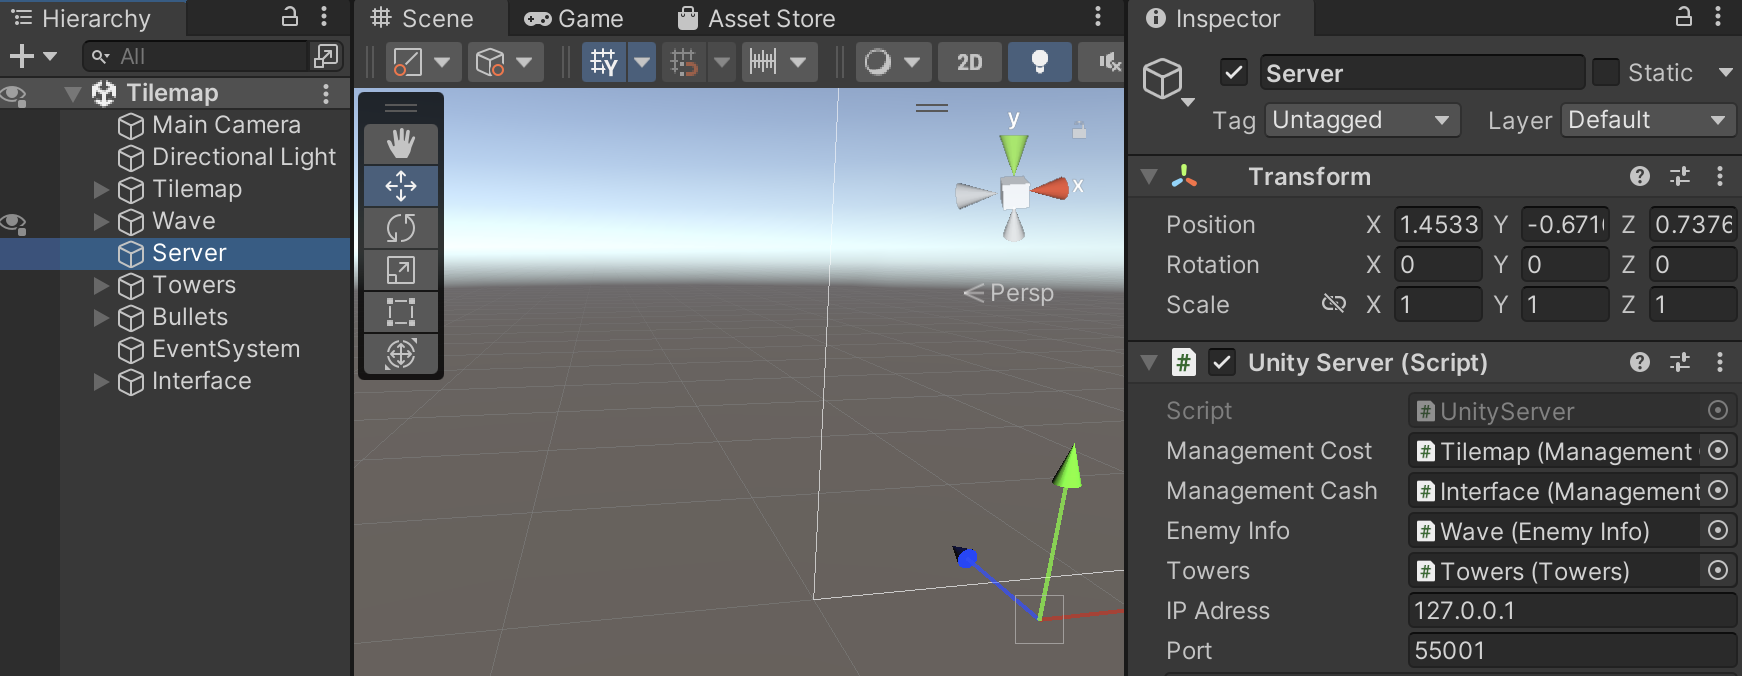
\includegraphics[width=15cm]{images/serverParameters.png}
\caption{Communication server parameters}
\label{Fig:serverParameters}
\end{figure} 

The game board is a set of $n \times m$ tiles with a square base. $n$ and $m$ are the width and height of the board, respectively, expressed in the lengths of the side of the square that is the base of the tile. Sample XML defining the game board:
\lstinputlisting[language=XML]{xml/tilemap.xml}

After sending the data, information is returned in the form of XML. In the case of game board definition, XML data is returned with information about the correctness (or not) of the information sent to the server:
\lstinputlisting[language=XML]{xml/tilemapResponse.xml}

XML defining opponent parameters:
\lstinputlisting[language=XML]{xml/enemy.xml}

After defining the parameters, information is returned about the correctness of the command execution (same as in the case of tilemap).

XML defining tower parameters:
\lstinputlisting[language=XML]{xml/tower.xml}

After defining the parameters, information is returned about the correctness of the command execution (same as in the case of tilemap).

Creating an opponent and releasing him along the selected path:
\lstinputlisting[language=XML]{xml/addEnemy.xml}

After creating an opponent, information is returned about the correctness of the command execution (same as in the case of tilemap).

XML to add a new tower:
\lstinputlisting[language=XML]{xml/addTower.xml}

After adding a new tower, information is returned about the correctness of the command execution (same as in the case of tilemap).

Request to send track information:
\lstinputlisting[language=XML]{xml/GetChoiceOfPathData.xml}

Information returned by the server:
\lstinputlisting[language=XML]{xml/GetChoiceOfPathDataResponse.xml}

Request for detailed game status information:
\lstinputlisting[language=XML]{xml/LevelData.xml}

Information returned by the server:
\lstinputlisting[language=XML]{xml/LevelDataResponse.xml}